\newpage
\subsection{Учет технологической оснастки }
\label{bp:rigging}
%
Технологическая оснастка необходима для изготовления готовой продукции. Заказ ФПФ производится у  сторонних производителей: ООО ''АРТМАШ ГРУПП'' и ООО ''ТМ-Москва''. Штанцевальные формы производятся самостоятельно, но в редких случаях возможен заказ у ООО «РАСТР—технология» или ООО «ЛАЗЕРПАК».   

При получении требований от клиента менеджер узнает о необходимости использования оснастки при производстве продукции. Возможность изготовления нового изделия на производстве определяет менеджер. В случае сомнения изготовления изделия менеджер согласует возможность с технологическим отделом.
%Если МСЗ сомневается в возможности производства продукции, он задает вопрос на производство инженеру-технологу или директору по  производству. 

\textbf{Учет печатных форм}

Менеджер создает заявку в технологический отдел на создание макета по электронной почте, исходные данные для макета предоставляет заказчик. Технолог по подготовке производства при необходимости дополняет заявку и отправляет ее по электронной почте производителю оснастки (рис. \ref{pic:II.8.3}). Изготовитель оснастки после создания макета высылает его технологу по подготовке производства (рис. \ref{pic:II.8.4}) для проверки. Далее макет пересылается контрагенту на согласование. После получения от контрагента согласованного макета технолог по подготовке производства создает  заявку на изготовление оснастки. Клише приходит с документами. Технолог по подготовке производства производит осмотр и прием оснастки и подписывает выставленный счет (рис. \ref{pic:II.8.9}). Технолог по подготовке производства передает документы в бухгалтерию для оформления поступления ТМЦ. Специалист по подготовке производства размещает оснастку в ячейке для хранения (рис. \ref{pic:II.5.7.}).  

%Предприятие использует одного поставщика флекс-форм. 
%Для заказа флекс-формы художник-конструктор использует согласованный дизайн макет, отправляет его по емайл.%, заявку на изготовление флекс-формы. 
%МСЗ и МАП проверяют внешний вид печати в файле согласованной технологической карты.

%Учет заявок на изготовление печатных флекс-форм не ведется. 
%При изготовлении печатной флекс-формы за счет клиента менеджер выставляет счет на изготовление оснастки.

%При поступлении на производство оснастка не проверяется. 

%Номер печатной формы присваивает участок вырубных форм на производстве в момент первого запуска и при нахождении свободной ячейки для хранения . 

%Ремонтом флекс-форм занимаются в основном на УВФ.

%На предприятии выделено место хранения флекс-форм (рис.  %, 32, 33
%При поступлении оснастки МСЗ принимает ее совместно с комплектовщиком, проверяют качество, присваивают номер.
%Номер определяется по файлу в формате MS Excel, где ведется список используемых на предприятии флекс-форм.

%После принятия к учету флекс-форм МСЗ сообщает дизайнеру о поступлении устно или через мессенджеры о необходимости добавления номера поступившей оснастки в разработанную технологическую карту.
%Комплектовщик принимает флекс-форму и размещает в ячейке для хранения. Место хранения флексо-форм  разделено по линиям (\ref{pic:a15}).  


\textbf{Учет штанцевальных форм.}

Менеджер создает заявку на изготовление оснастки и направляет по электронной почте технологу по подготовке производства. Перед началом изготовления штанцевальной формы создается чертеж образца изготовляется образец на плоттере. Образец изделия и чертеж направляются клиенту на согласование. После согласования с клиентом, технолог по подготовке производства оформляет заявку на изготовление штанцевальной формы и мастера по ремонту и изготовлению оснастки изготавливают оснастку. Технолог по подготовке производства принимает штанцевальную форму. Специалист по подготовке производства определяет место хранения и размещает оснастку у соответствующей линии (рис. \ref{pic:II.5.7}).  
%На предприятии используются только роторные штанцевальные формы.
Любым ремонтом оснастки занимаются мастера по ремонту и изготовлению оснастки.
%Клиент предоставляет макет по изготовлению изделия для сложных изделий. Дизайнер на предприятии не разрабатывает макет высекательных штанцевальных форм.
Журналы выдачи оснастки не ведутся. Вся оснастка находится у линий переработки.

 \textbf{Учет краски}.

 Краска приобретается в виде пигментов. В системе 1С: УПП технологическим отделом  оформляется документ ''Заказ поставщику''. Поставщик присылает счет на оплату. Краска принимается технологом по подготовке производства. Далее все документы передаются в бухгалтерию.  








\clearpage



\begin{figure}
\begin{center}
 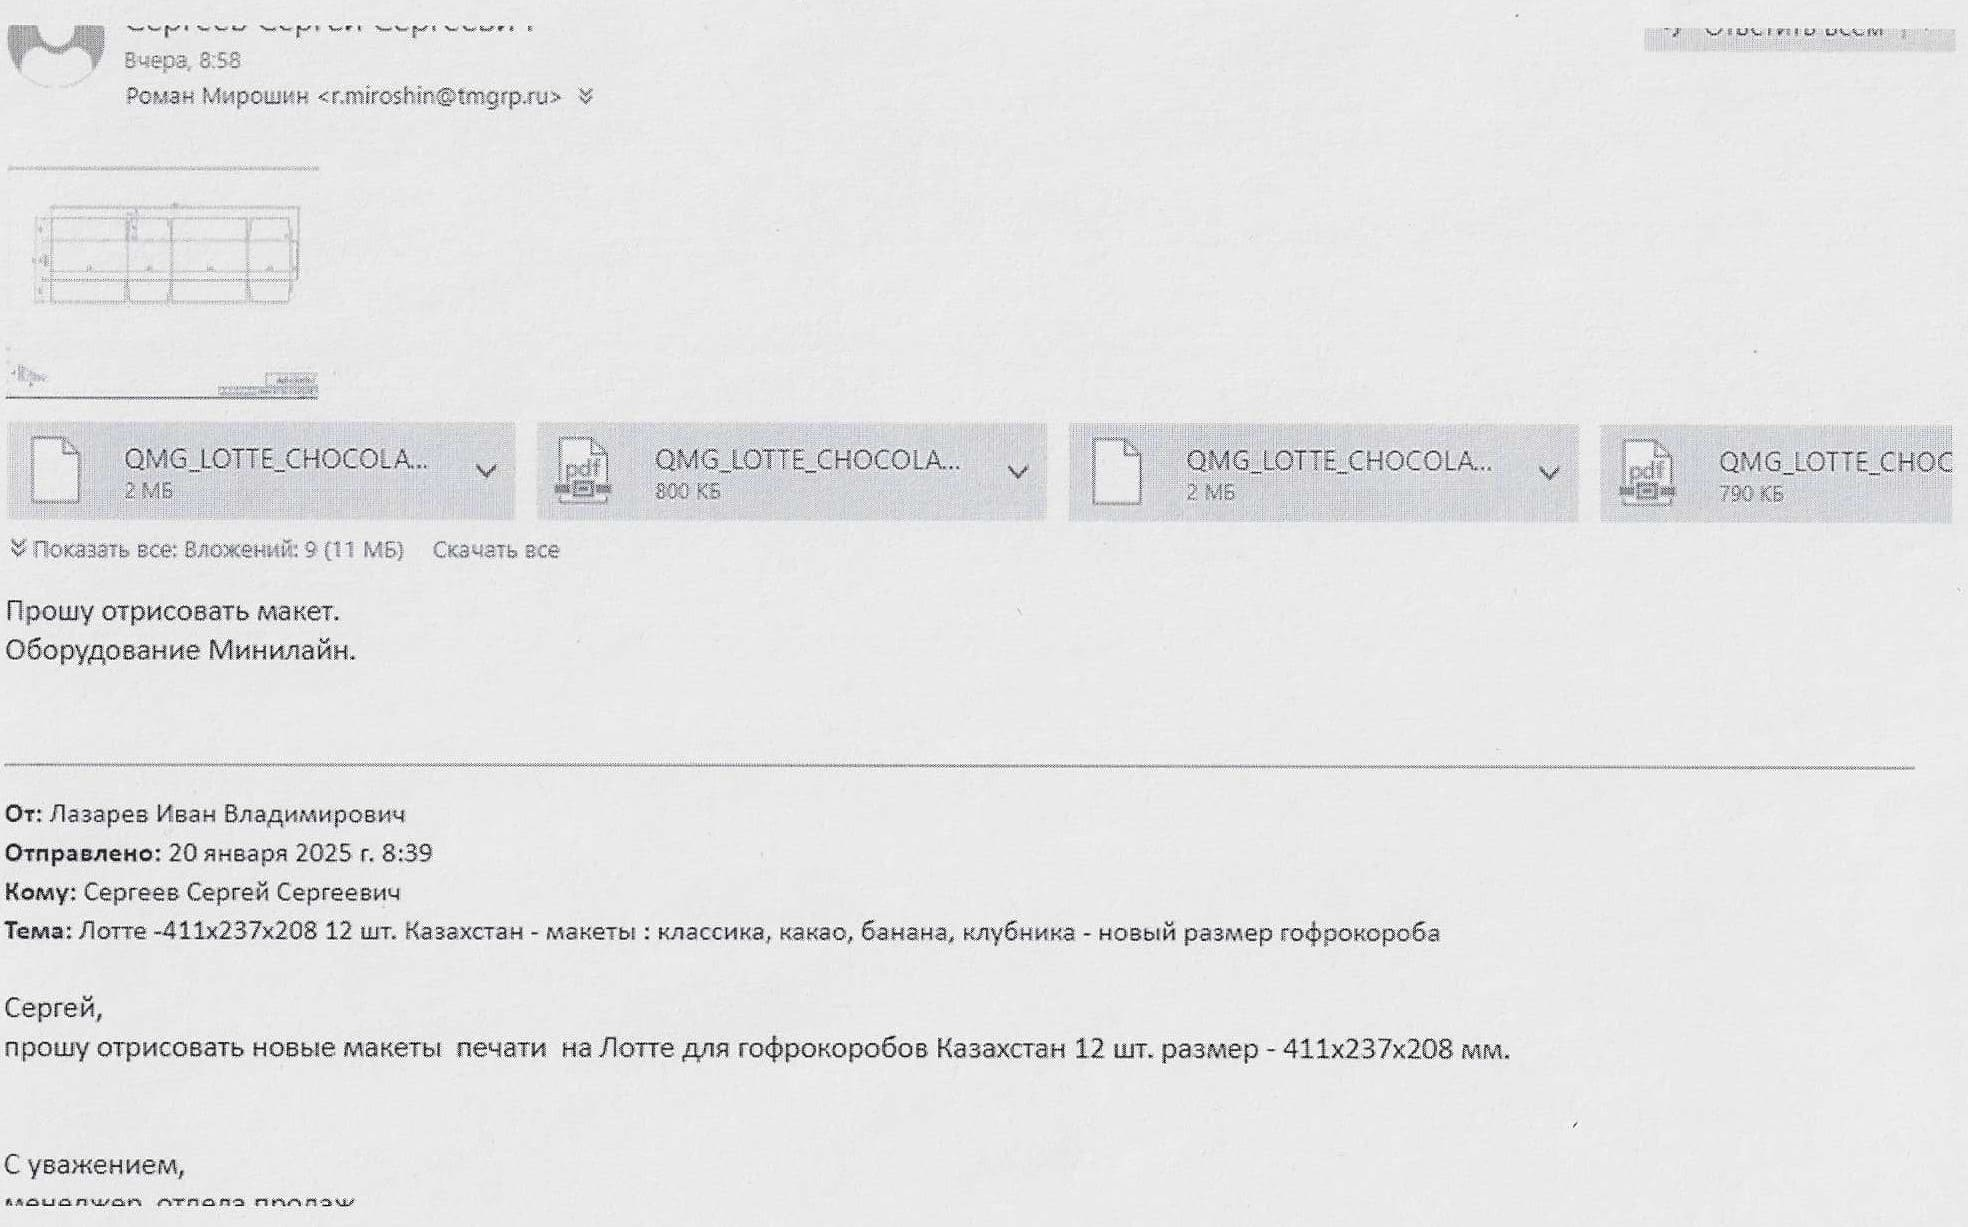
\includegraphics[height=0.4\textheight, keepaspectratio]{Pics/II.8.3.jpg}
\end{center}
 \caption{Заявка на макет производителю}
 \label{pic:II.8.3}
\end{figure}

\begin{figure}
\begin{center}
 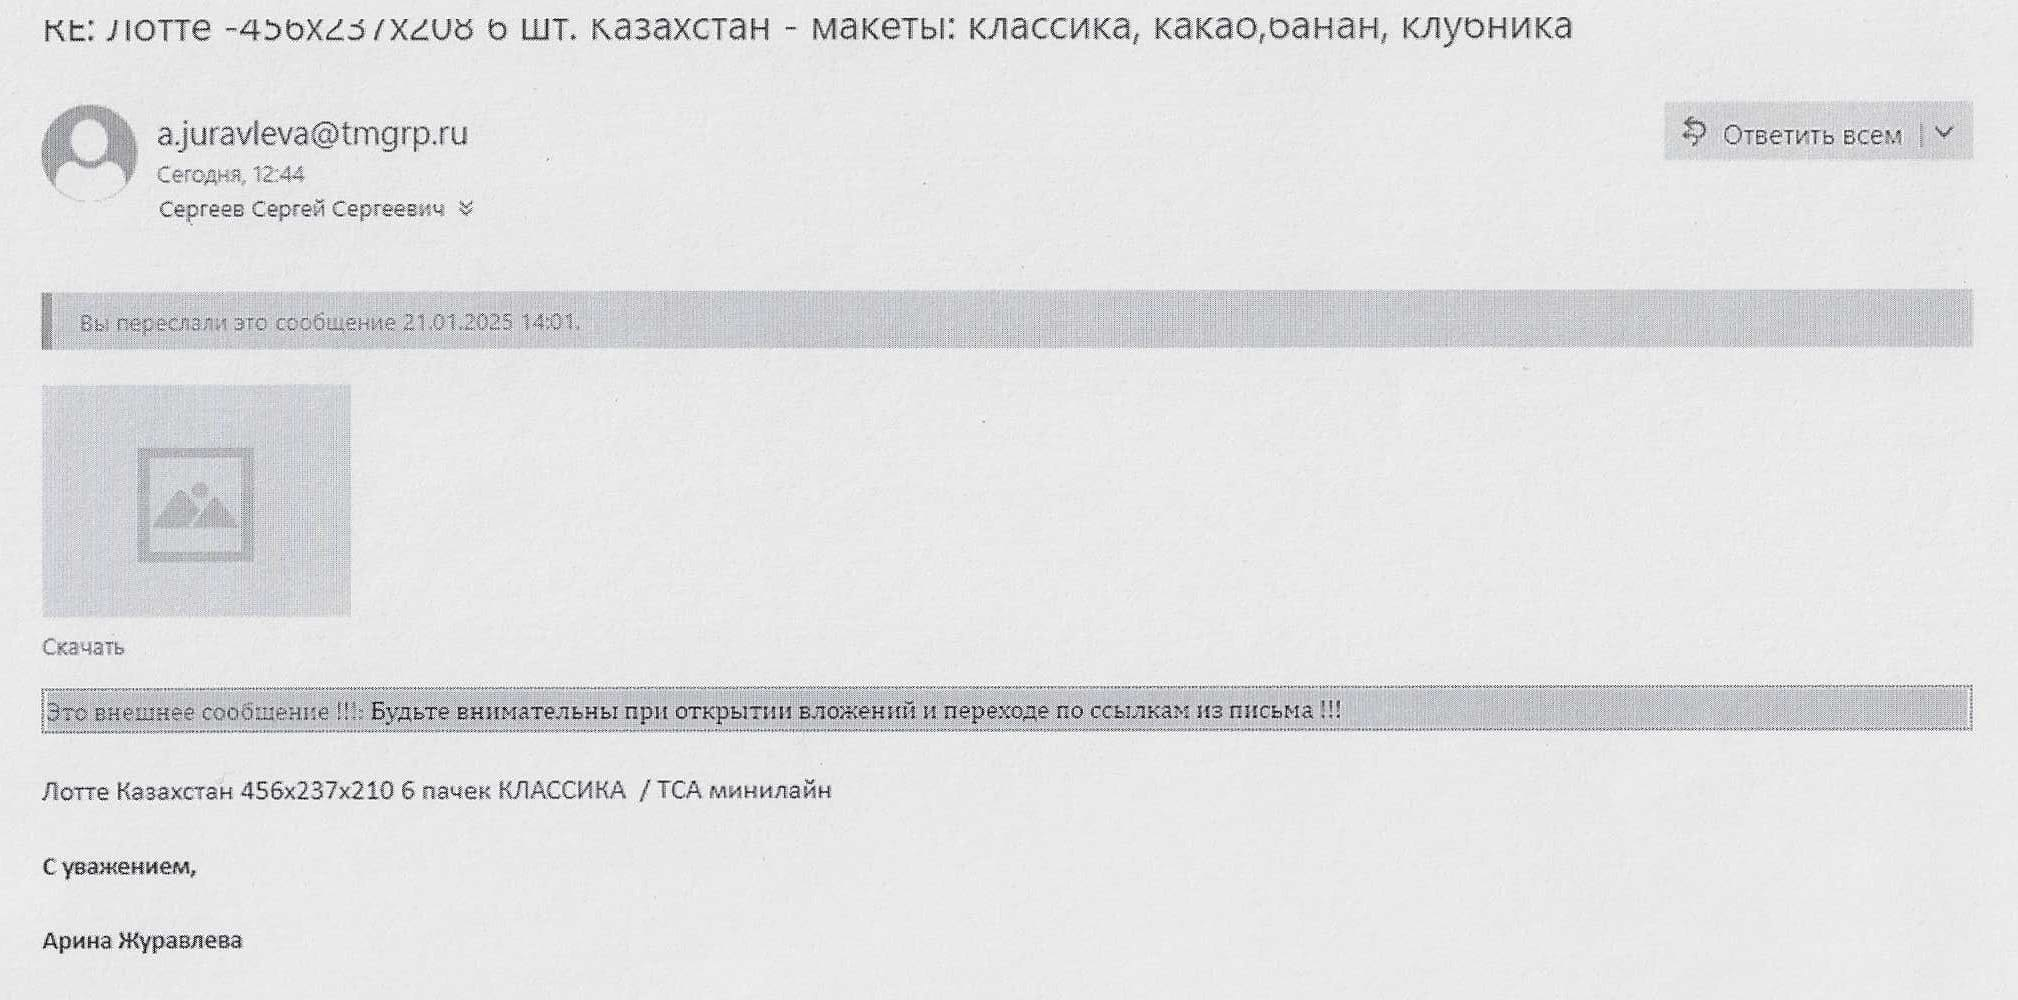
\includegraphics[height=0.3\textheight, keepaspectratio]{Pics/II.8.4.jpg}
\end{center}
 \caption{Ответ производителя оснастки}
 \label{pic:II.8.4}
\end{figure}

%\begin{figure}
%\begin{center}
% 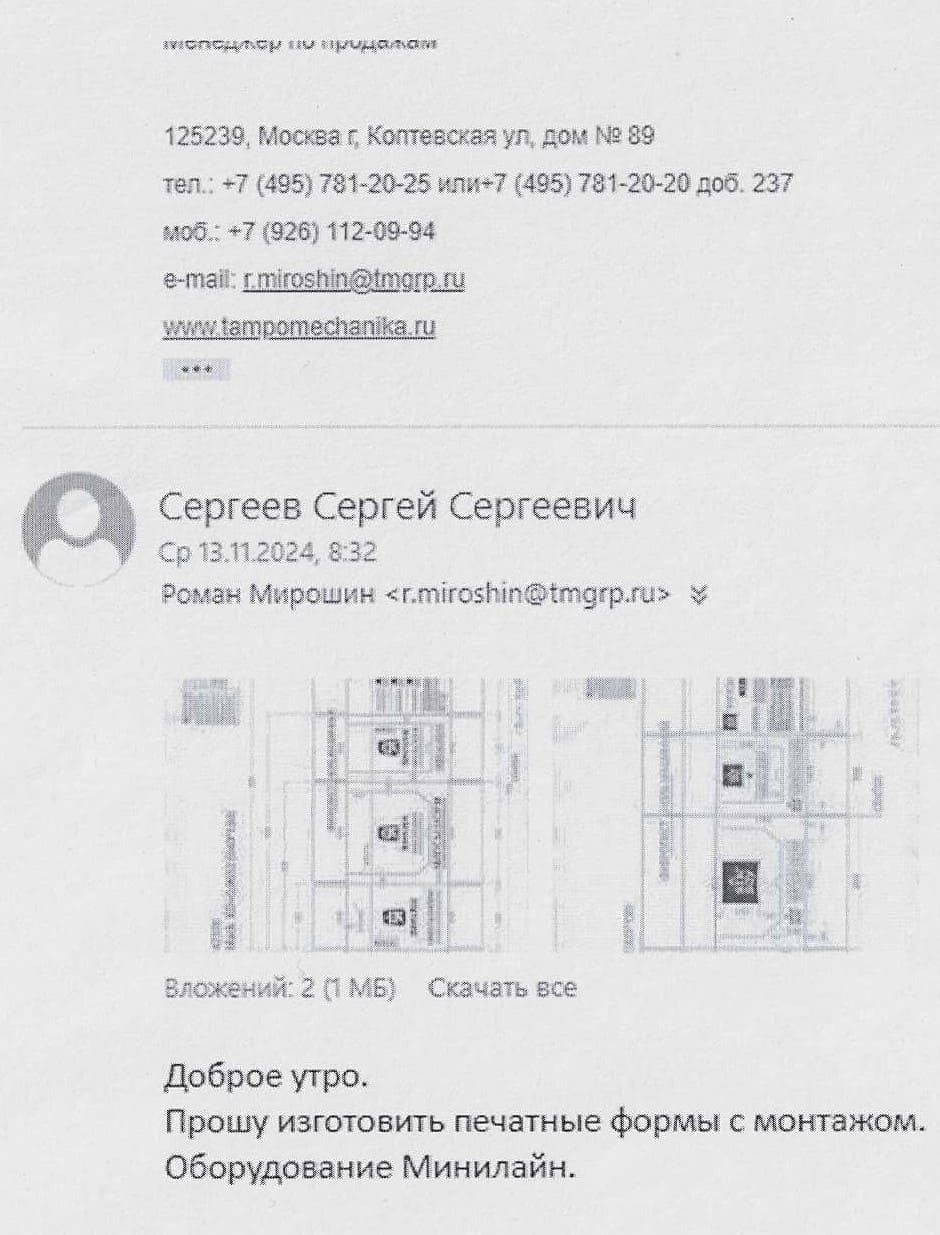
\includegraphics[height=0.45\textheight, keepaspectratio]{Pics/II.8.7.jpg}
%\end{center}
 %\caption{Заявка на изготовление оснастки}
 %\label{pic:II.8.7}
%\end{figure}

\begin{figure}
\begin{center}
 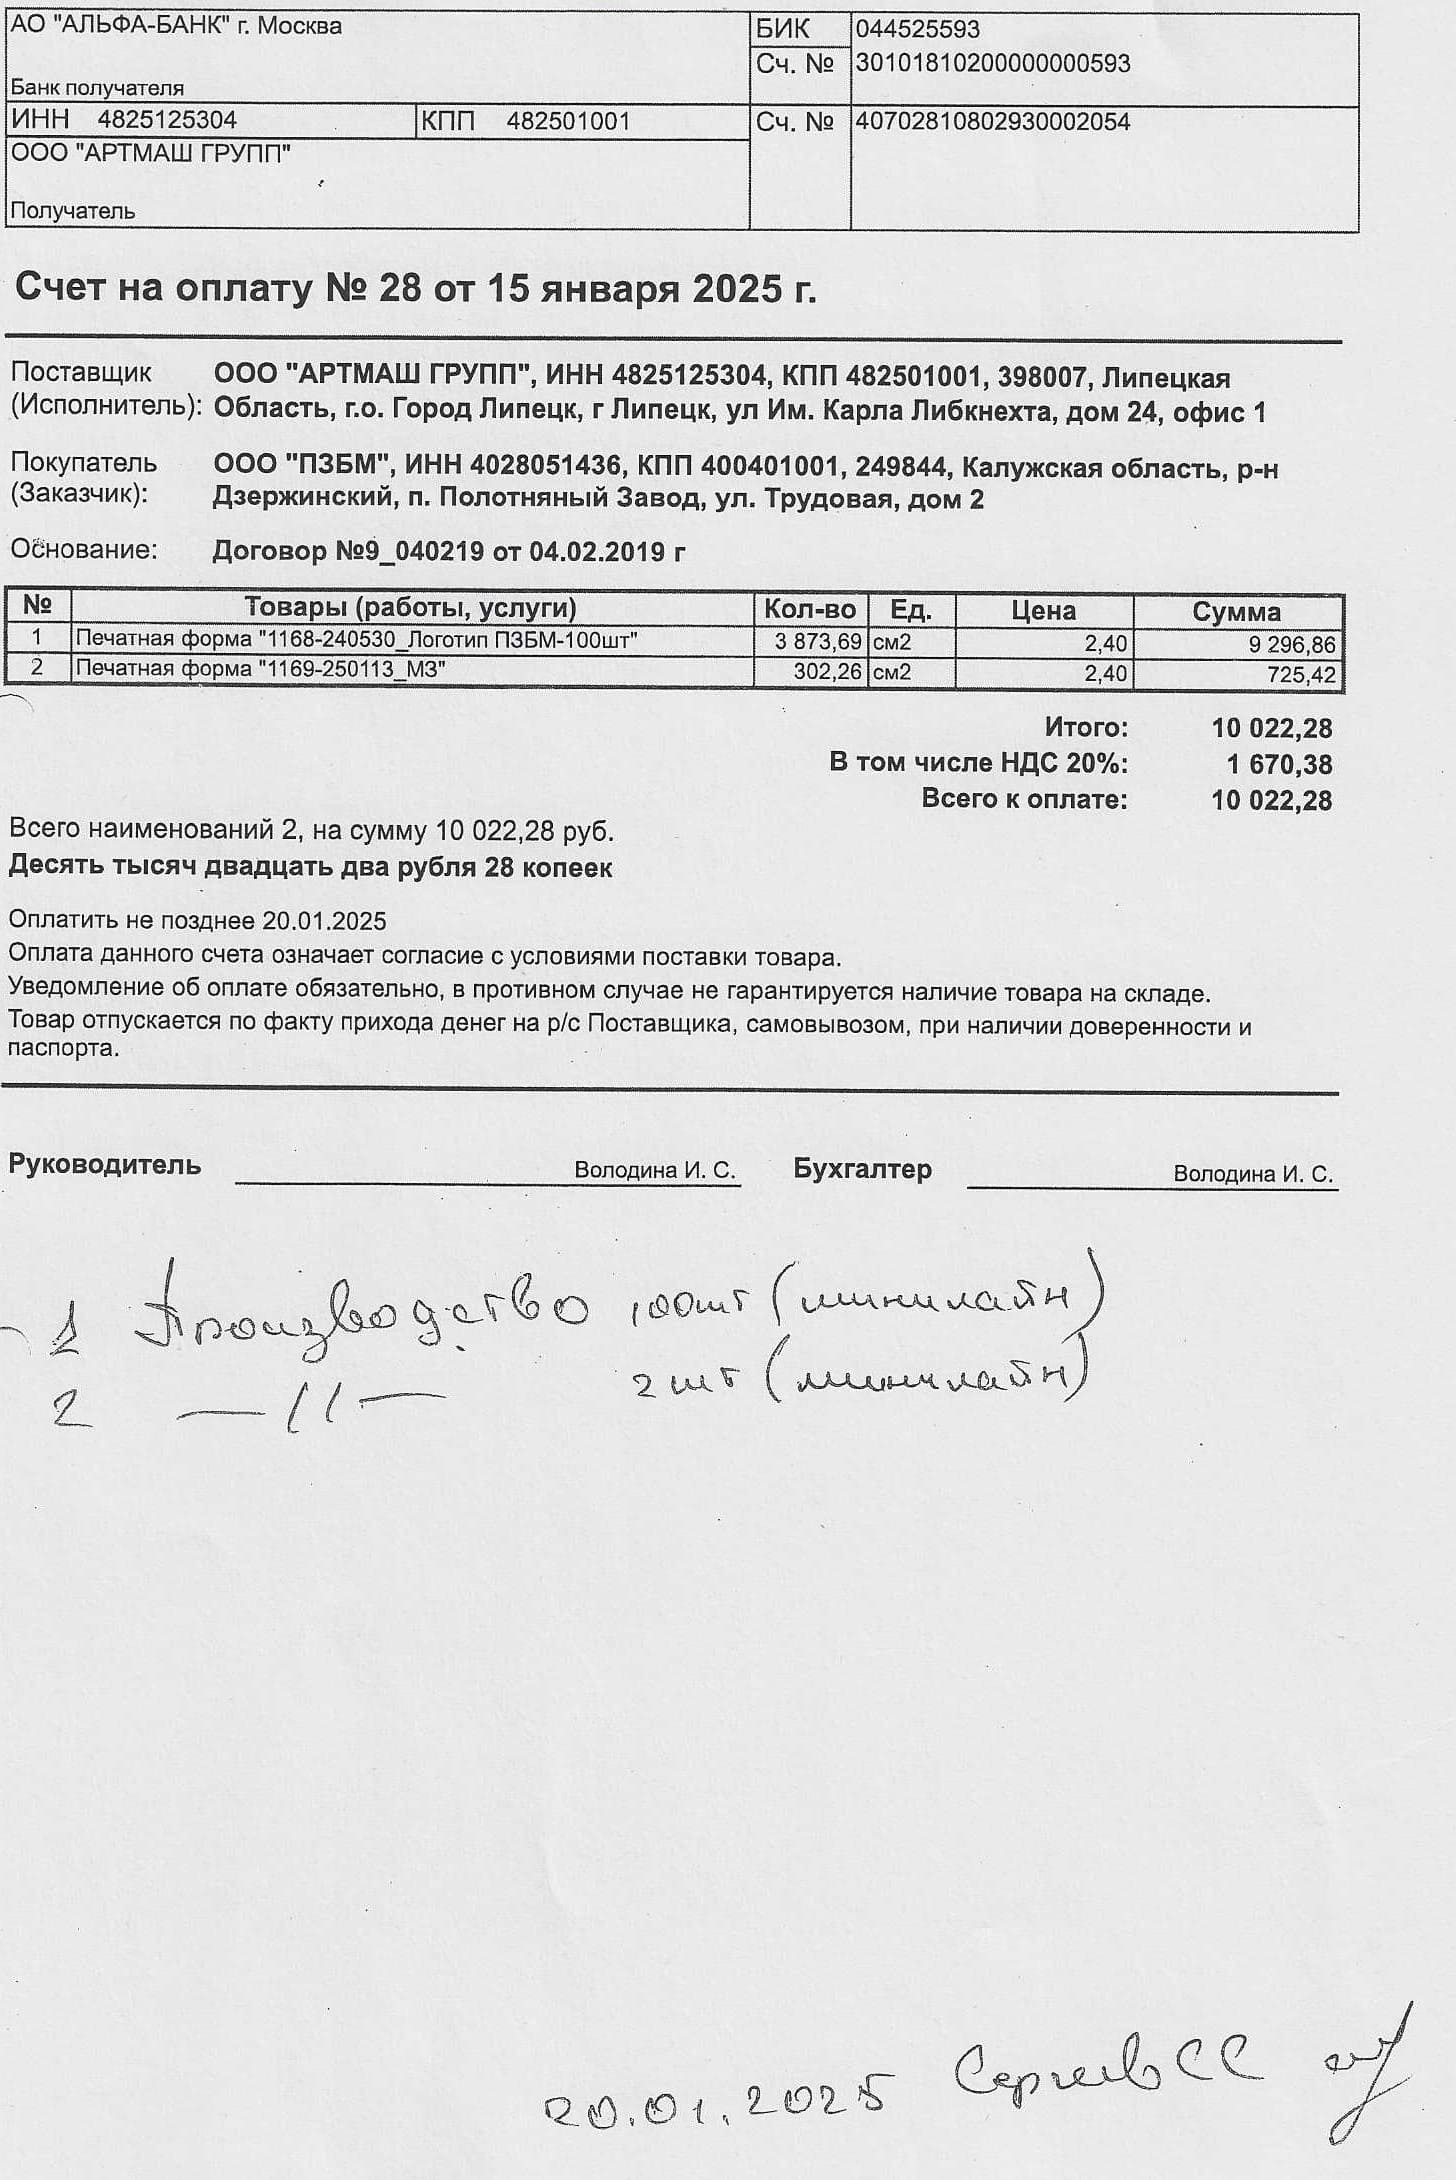
\includegraphics[height=0.9\textheight, keepaspectratio]{Pics/II.8.9.jpg}
\end{center}
 \caption{Счет на оснастку}
 \label{pic:II.8.9}
\end{figure}


\begin{figure}
\begin{center}
 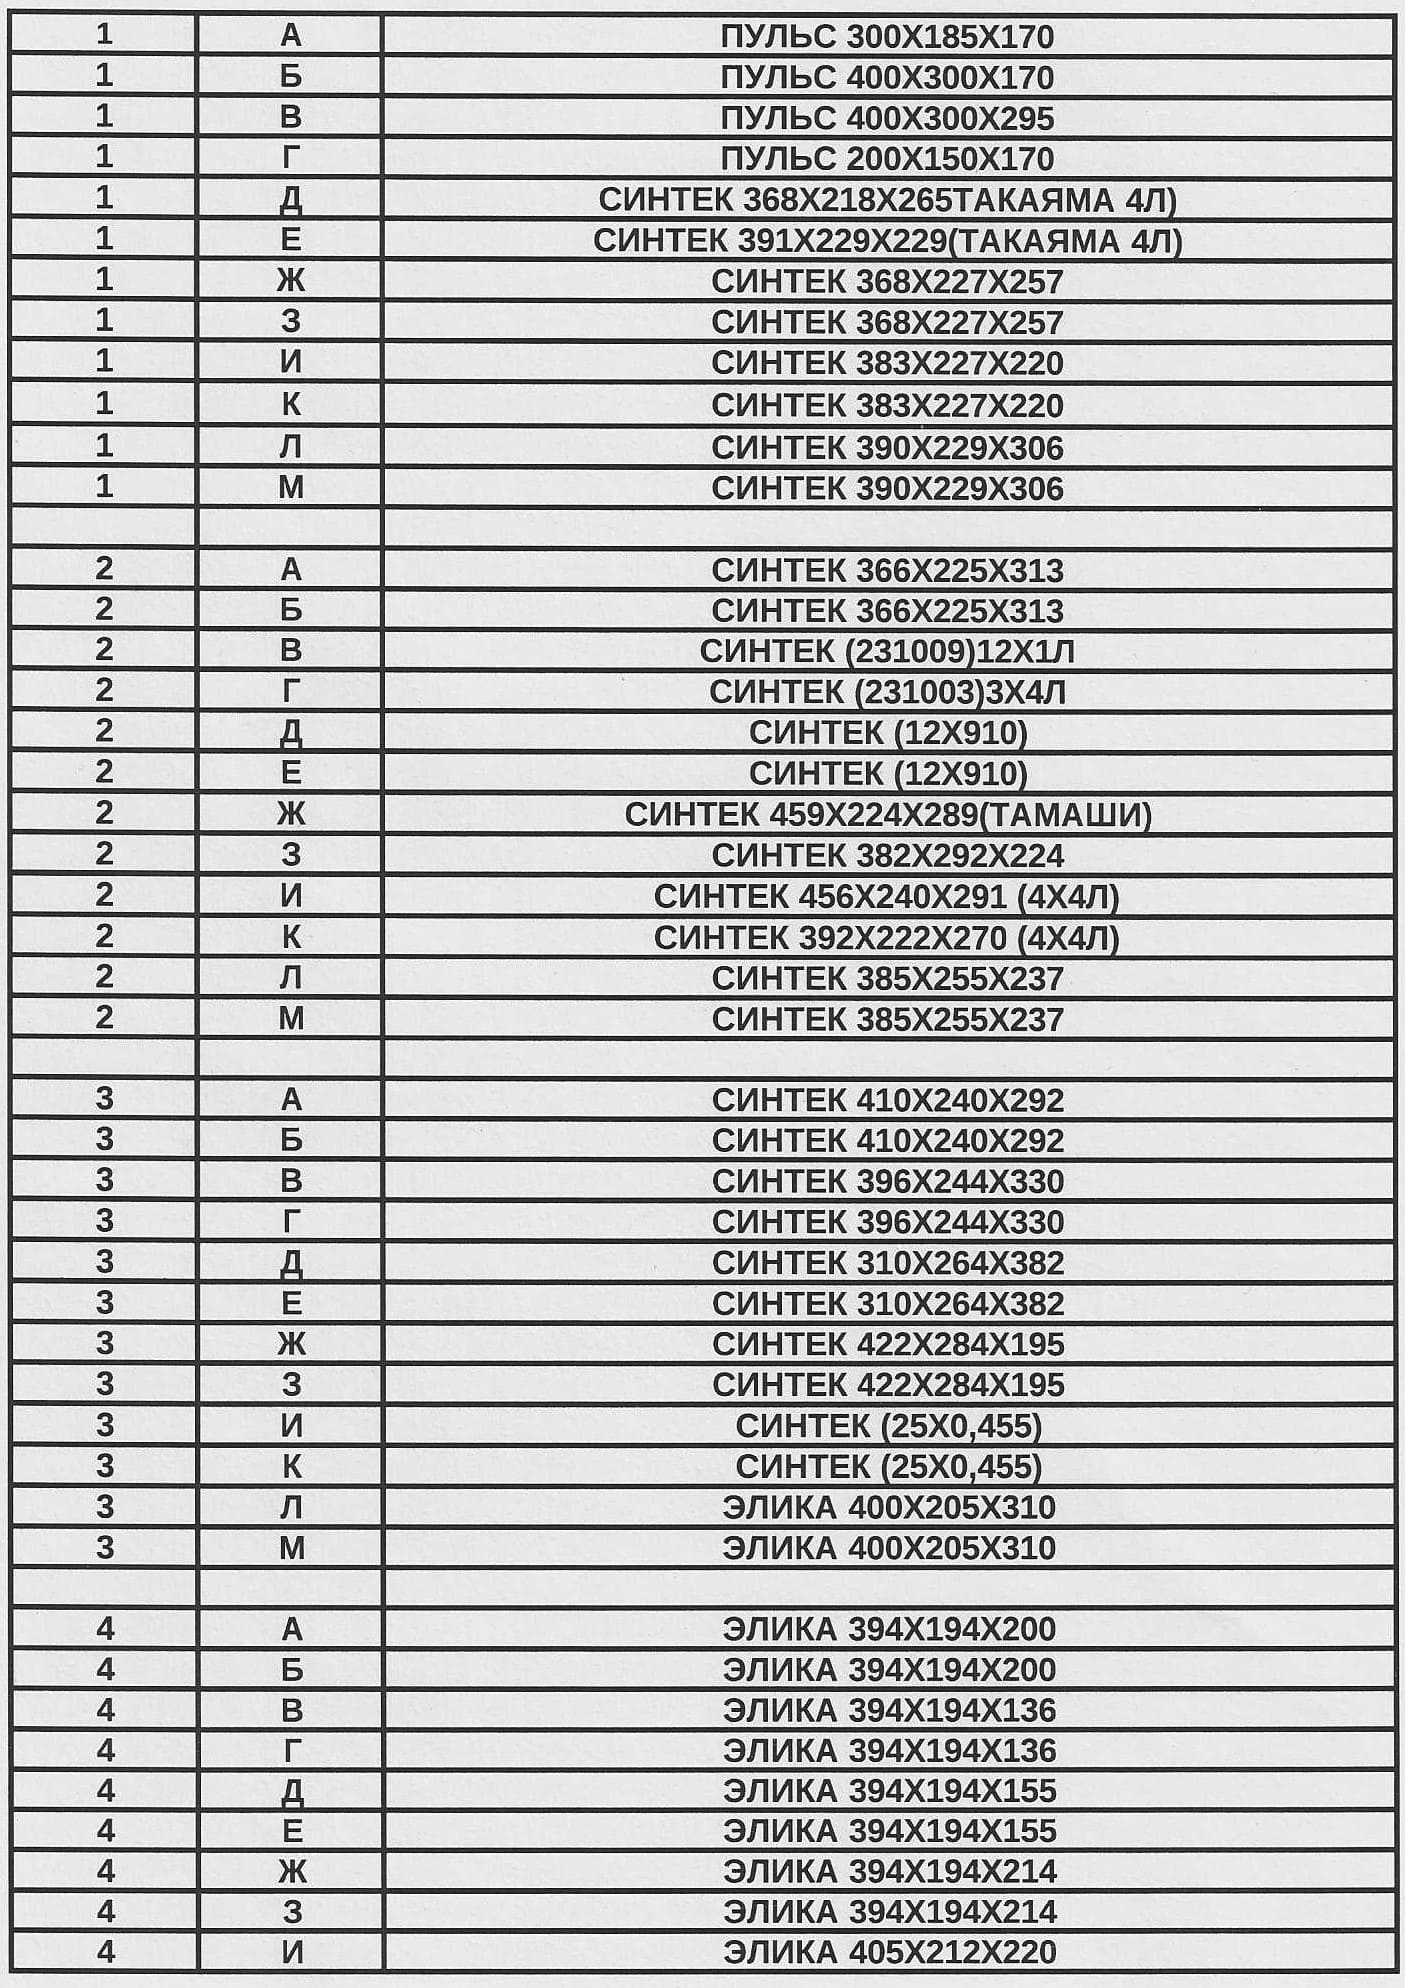
\includegraphics[height=0.7\textheight, keepaspectratio]{Pics/II.5.7..jpg}
\end{center}
 \caption{Ячейки для хранения оснастки}
 \label{pic:II.5.7.}
\end{figure}


\begin{figure}
\begin{center}
 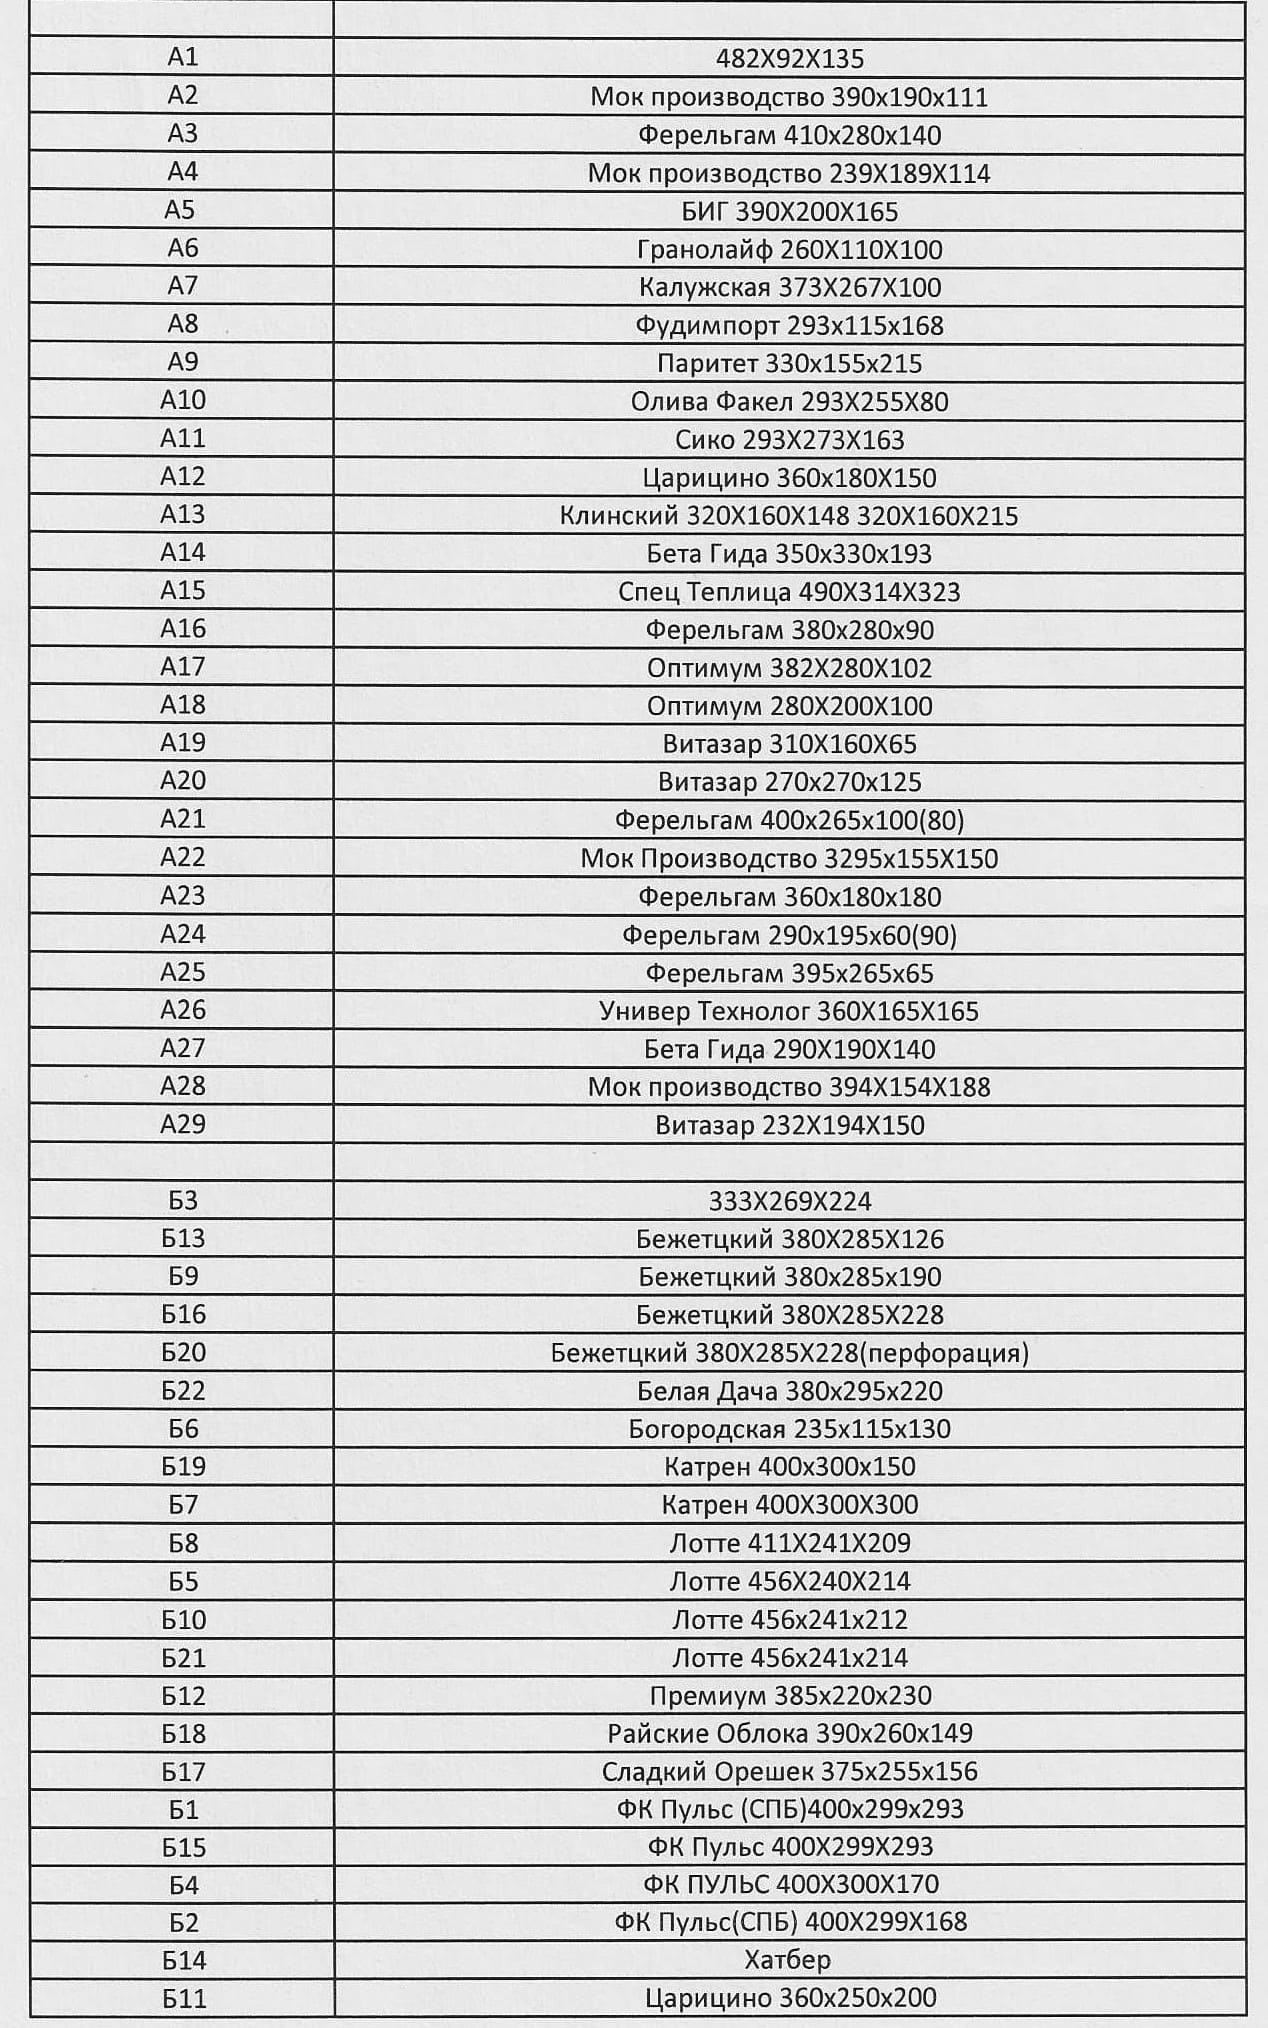
\includegraphics[height=0.8\textheight, keepaspectratio]{Pics/II.5.7.jpg}
\end{center}
 \caption{Ячейки для хранения оснастки}
 \label{pic:II.5.7}
\end{figure}

\clearpage
% \begin{figure}
% \begin{center}
%   \includegraphics[height=0.94\textheight, width=0.94\textwidth, keepaspectratio]{Pics/a7.jpg}
% \end{center}
%   \caption{Отчет по краске в системе}
%   \label{pic:a7}
% \end{figure}

% \begin{figure}
% \begin{center}
%   \includegraphics[height=0.94\textheight, width=0.94\textwidth, keepaspectratio]{Pics/a9.jpg}
% \end{center}
%   \caption{Отчет по поступлению краски}
%   \label{pic:a9}
% \end{figure}





% \begin{figure}
% \begin{center}
%   \includegraphics[height=0.94\textheight, width=0.94\textwidth, keepaspectratio]{Pics/pic_d41.jpg}
% \end{center}
%   \caption{Форма  оснастки монтажистам}
%   \label{pic:pic_d41}
% \end{figure}
% \clearpage
%
% 

\clearpage
\ifx \notincludehead\undefined
\normalsize
\end{document}
\fi
